\usetikzlibrary{arrows.meta,calc}
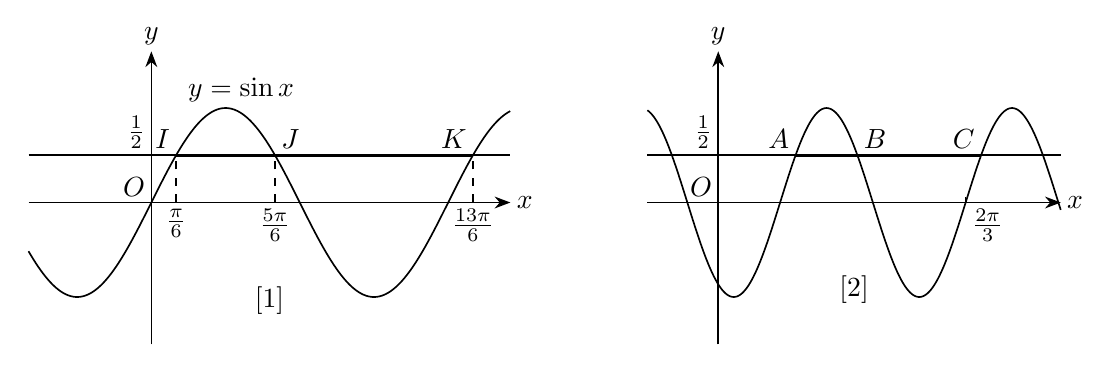
\begin{tikzpicture}[line width=.6pt,>=Stealth,font=\normalsize]
% ---- left panel 图1: y=sin x ----
\begin{scope}[x=0.6cm,y=1.2cm]
\draw[->] (-2.6,0)--(7.6,0) node[right,inner sep=0pt,xshift=2pt] {$x$};
\draw[->] (0,-1.5)--(0,1.6) node[above,inner sep=0pt,yshift=2pt] {$y$};
\node[above left,inner sep=0pt,xshift=-2pt,yshift=2pt] at (0,0) {$O$};
\draw[line width=.6pt] (0,0.5)--(0.07,0.5);
\node[above left,inner sep=0pt,xshift=-2pt,yshift=2pt] at (0,0.5) {$\frac12$};
\draw[domain=-2.6:7.6,samples=280] plot (\x,{sin(deg(\x))});
\draw (-2.6,0.5)--(7.6,0.5);
% thick subsegment I-K along y=1/2 (grayscale emphasis)
\draw[line width=1.1pt] (0.52359878,0.5)--(6.80678408,0.5);
% droplines
\draw[dashed] (0.52359878,0)--(0.52359878,0.5);
\draw[dashed] (2.61799388,0)--(2.61799388,0.5);
\draw[dashed] (6.80678408,0)--(6.80678408,0.5);
% x ticks below axis
\node[below,inner sep=0pt,yshift=-2pt] at (0.52359878,0) {$\frac{\pi}{6}$};
\node[below,inner sep=0pt,yshift=-2pt] at (2.61799388,0) {$\frac{5\pi}{6}$};
\node[below,inner sep=0pt,yshift=-2pt] at (6.80678408,0) {$\frac{13\pi}{6}$};
% I,J,K above line, diagonal offsets to clear steep sine
\node[above left,inner sep=0pt,xshift=-2pt,yshift=2pt] at (0.52359878,0.5) {$I$};
\node[above right,inner sep=0pt,xshift=2pt,yshift=2pt] at (2.61799388,0.5) {$J$};
\node[above left,inner sep=0pt,xshift=-2pt,yshift=2pt] at (6.80678408,0.5) {$K$};
\node[above,inner sep=0pt,yshift=2pt] at (1.9,1.0) {$y=\sin x$};
\node[below,inner sep=0pt,yshift=-30pt] at (2.5,0) {\bitmapinsertcaption[1]};
\end{scope}
% ---- right panel 图2: omega-4 sine ----
\begin{scope}[x=1.5cm,y=1.2cm,shift={(7.2cm,0cm)}]
\draw[->] (-0.6,0)--(2.9,0) node[right,inner sep=0pt,xshift=2pt] {$x$};
\draw[->] (0,-1.5)--(0,1.6) node[above,inner sep=0pt,yshift=2pt] {$y$};
\node[above left,inner sep=0pt,xshift=-2pt,yshift=2pt] at (0,0) {$O$};
\draw[line width=.6pt] (0,0.5)--(0.06,0.5);
\node[above left,inner sep=0pt,xshift=-2pt,yshift=2pt] at (0,0.5) {$\frac12$};
\draw[domain=-0.6:2.9,samples=250] plot (\x,{sin(4*deg(\x)-480)});
\draw (-0.6,0.5)--(2.9,0.5);
\draw[line width=1.1pt] (0.65449847,0.5)--(2.2252948,0.5);
\draw[line width=.6pt] (2.0943951,0)--(2.0943951,0.06);
\node[below right,inner sep=0pt,xshift=2pt,yshift=-2pt] at (2.0943951,0) {$\frac{2\pi}{3}$};
\node[above left,inner sep=0pt,xshift=-2pt,yshift=2pt] at (0.65449847,0.5) {$A$};
\node[above right,inner sep=0pt,xshift=2pt,yshift=2pt] at (1.17809725,0.5) {$B$};
\node[above left,inner sep=0pt,xshift=-2pt,yshift=2pt] at (2.2252948,0.5) {$C$};
\node[below,inner sep=0pt,yshift=-26pt] at (1.15,0) {\bitmapinsertcaption[2]};
\end{scope}
\end{tikzpicture}
